\documentclass[12pt]{beamer}
\usetheme{LSU}
%\hypersetup{pdfpagemode=FullScreen}

\setbeamertemplate{footline}[text line]{} % makes the footer EMPTY
\useoutertheme[subsection=false]{smoothbars}

\usepackage{subfigure}
\usepackage{multicol}
\usepackage{graphicx}
\usepackage[all,knot]{xy}
\usepackage{url}
\usepackage{multimedia}
\usepackage{hyperref}
\usepackage{xcolor}
\usepackage{tabularx}

\usefonttheme{professionalfonts}
\usefonttheme{serif}
\usepackage{fontspec}
\setmainfont{Ubuntu}


\title{\Large What is ecology?}
\author{LSU -- Biol 4253}
\date{}





\begin{document}

\maketitle




% Go over syllabus, expectations, course project, grading, textbook, etc.


%%%%% structure of lecture:



% What is ecology? --study of species interactions (intraspecific interactions, interspecific interactions, interactions with abiotic environment, etc.)


\begin{frame}

	\begin{flushright}
	  \Large \textcolor{boss2}{Ecology} 
	\end{flushright}
\end{frame}






% Edit with pretty pictures to elaborate on each one of these.

\begin{frame}

	\begin{flushright}
	  {\Large \textcolor{boss2}{Species interactions!}}
	\end{flushright}

  With other species:
  \begin{itemize}
    \item Competition
    \item Predator -- prey
    \item Plant -- pollinator
    \item Host -- parasite
  \end{itemize}  

\end{frame}




\begin{frame}

	\begin{flushright}
	  {\Large \textcolor{boss2}{Species interactions!}}
	\end{flushright}

  With the environment:
  \begin{itemize}
    \item Abiotic variables
    \item Dispersal limitation
    \item Ecosystem respiration 
    \item Ecosystem engineering
  \end{itemize}  
\end{frame}
















% What isn't ecology?



\begin{frame}

  {\Large  \textcolor{boss1}{What is not ecology?}} \\

\end{frame}





%Discuss these individually. What do they share in common, and how do they fundamentally differ?

\begin{frame}

	\begin{flushright}
	  \Large \textcolor{boss2}{Environmentalism} \\
	  \Large \textcolor{boss3}{Biomedicine} \\
	  \Large \textcolor{boss4}{Natural history} \\
	  \Large \textcolor{boss4}{Evolution} \\
	\end{flushright}
\end{frame}



\begin{frame}

	\begin{flushright}
	  \Large \textcolor{boss2}{} 
	\end{flushright}
\end{frame}




\begin{frame}

	\begin{flushright}
	  \Large \textcolor{boss2}{} 
	\end{flushright}
\end{frame}








































% Historical roots of ecology and where we are now. 

\begin{frame}

	\begin{flushright}
	  \Large \textcolor{boss2}{ } 
	\end{flushright}
\end{frame}


\begin{frame}

	\begin{flushright}
	  \Large \textcolor{boss2}{ } 
	\end{flushright}
\end{frame}



\begin{frame}

	\begin{flushright}
	  \Large \textcolor{boss2}{ } 
	\end{flushright}
\end{frame}



\begin{frame}

	\begin{flushright}
	  \Large \textcolor{boss2}{ } 
	\end{flushright}
\end{frame}


















% Levels of biological organization (individual, population, community, ecosystem)--drill down into each one of these.


\begin{frame}

  \textcolor{boss5}{Levels of biological organization}\\
  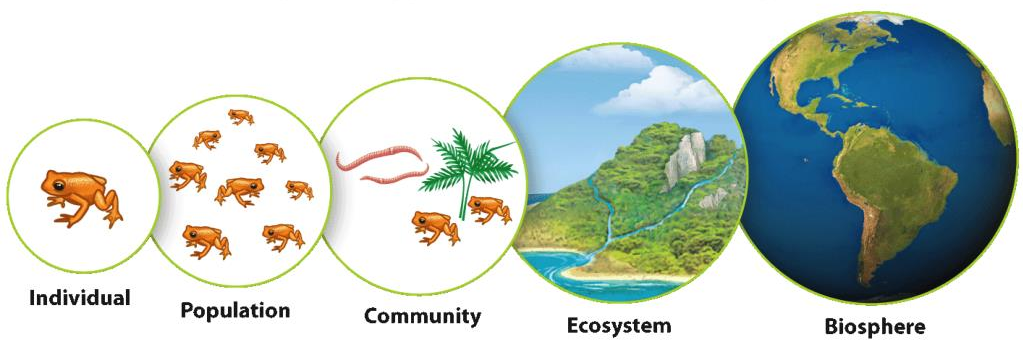
\includegraphics[width=\textwidth]{figs/ecologicalOrganization.png}
\end{frame}





\begin{frame}

	\begin{flushright}
	  \Large \textcolor{boss2}{Individual} 
	\end{flushright}
\end{frame}


\begin{frame}

	\begin{flushright}
	  \Large \textcolor{boss2}{Population} 
	\end{flushright}
\end{frame}




\begin{frame}

	\begin{flushright}
	  \Large \textcolor{boss2}{Community} 
	\end{flushright}
\end{frame}





\begin{frame}

	\begin{flushright}
	  \Large \textcolor{boss2}{Ecosystem} 
	\end{flushright}
\end{frame}


\begin{frame}

	\begin{flushright}
	  \Large \textcolor{boss2}{Biosphere} 
	\end{flushright}
\end{frame}





\begin{frame}

	\begin{flushright}
	  \Large \textcolor{boss2}{} 
	\end{flushright}
\end{frame}











\begin{frame}

{\large \textcolor{lsu1}{Contact info}}

  \begin{itemize}
    \item \textcolor{lsu2}{Office:} A343 Life Sciences
  \end{itemize}

  \begin{flushright}
    \begin{tabular}{cl}
    
\includegraphics[width=0.75cm]{figs/email.png} & \texttt{tadallas@lsu.edu} \\
    
\includegraphics[width=1.5cm]{figs/octocat.png} & \texttt{taddallas} \\
    
\includegraphics[width=0.75cm]{figs/user.png} & \texttt{taddallas.github.io}\\
   \end{tabular}
  \end{flushright}
\end{frame}



























% first class of the week is above, second class of the week is below. Try to keep this set up, where lecture is on the first meeting, and the second class period provides clear examples in a lab-like environment where I actively code examples and we discuss them. 


\begin{frame}

  \Large \textcolor{boss1}{An introduction to R}

\end{frame}







\begin{frame}

  \Large \textcolor{boss1}{The role of computing to ecology}

\end{frame}




% Point to repo of code and make sure students have link/access. 
\begin{frame}

  \Large \textcolor{boss1}{The role of R in this class}

\end{frame}






\begin{frame}

  \Large \textcolor{boss1}{Why R?}

\end{frame}







\begin{frame}

  \Large \textcolor{boss1}{Data structures}

\end{frame}




\begin{frame}

  \Large \textcolor{boss1}{Data structures}

\end{frame}














\end{document}
